\section{Cable management}
\label{sec:cable-menagement}
\begin{figure*}
    \centering
    \begin{subfigure}[t!]
        {0.3\textwidth}
        \centering
        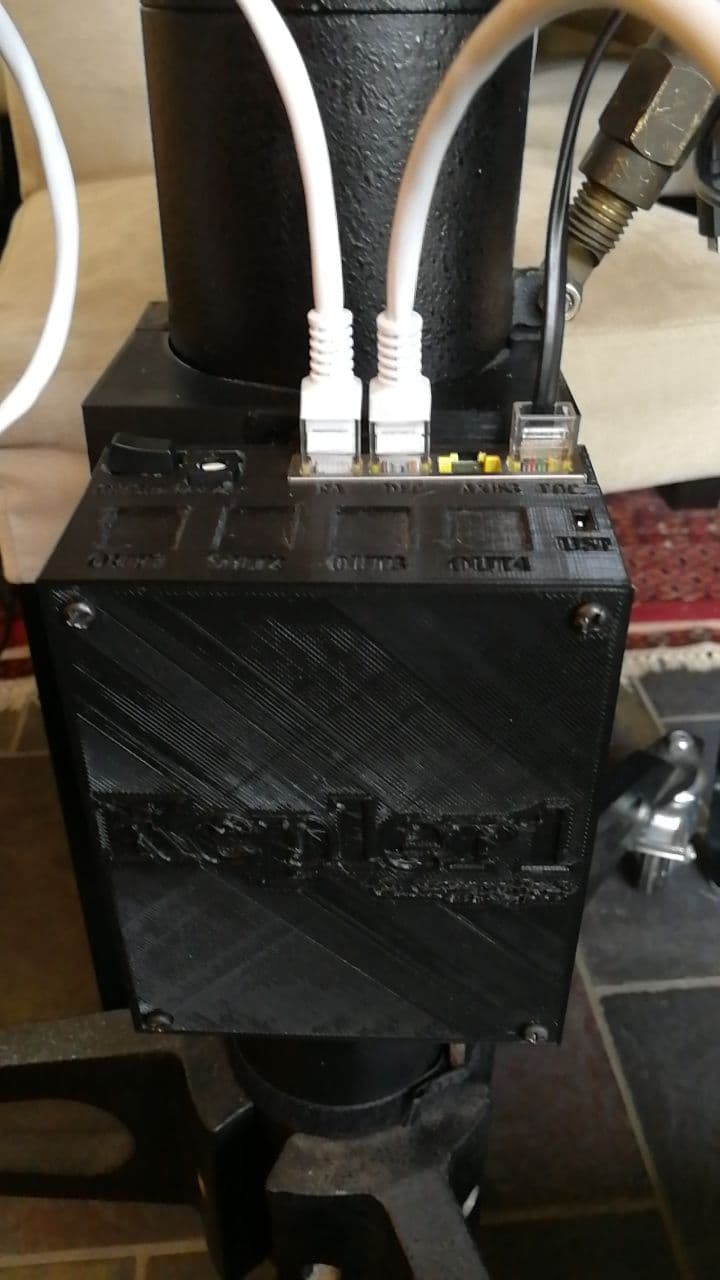
\includegraphics[scale=0.5]{BOX.jpg}
        \caption{The main box containing the electronics and its easy management Ethernet connections.}
        \label{fig:box}
    \end{subfigure}
    \begin{subfigure}[t!]
        {0.3\textwidth}
        \centering
        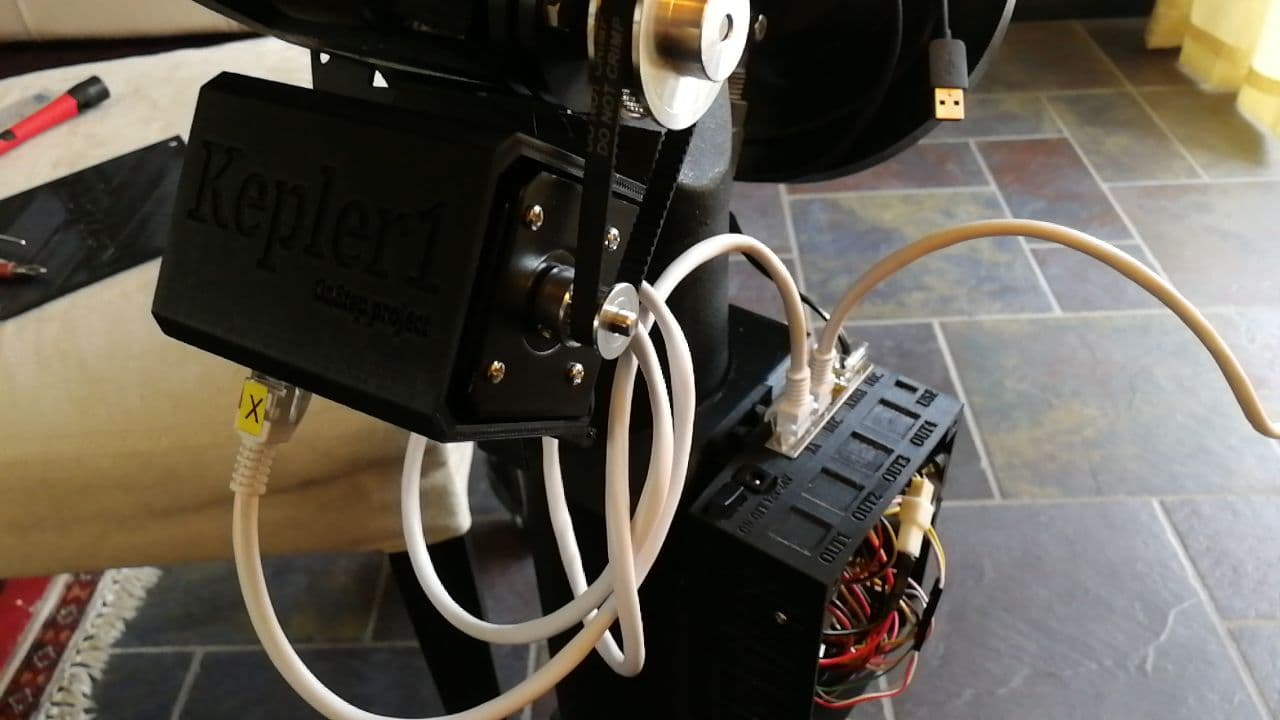
\includegraphics[scale=0.5]{RA-box.jpg}
        \caption{The RA motor box containing the stepper motor and its Ethernet socket.}
        \label{fig:RA-box}
    \end{subfigure}
    \begin{subfigure}[t!]
        {0.3\textwidth}
        \centering
        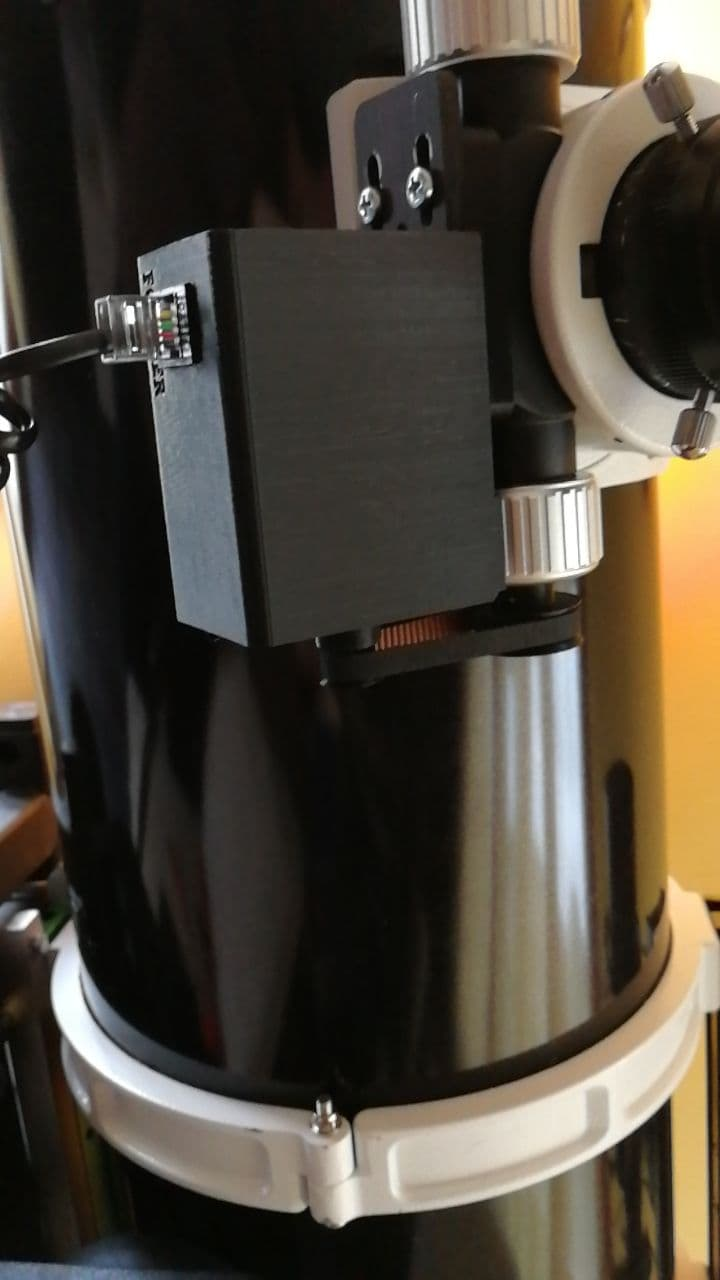
\includegraphics[scale=0.5]{FOCUSER-box.jpg}
        \caption{The focuser box containing the focuser stepper motor and its Ethernet socket.}
        \label{fig:focuser-box}
    \end{subfigure}
    \caption{Plastic boxes.}
    \label{fig:plastic-boxes}
\end{figure*}
The wiring between the electronics and the motors is made focusing on the main idea to attach and detach them rapidly.
We thought to use Ethernet cables.
They are a versatile solution but how to connect them to the four cables governing the stepper motor?

Stepper motors have four cables, see figure \ref{fig:stepper-motors-cables}, which have to be driven to the CNC3.
\\
\begin{minipage}
    {0.5\textwidth}
    \centering
    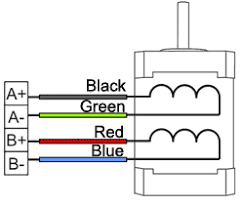
\includegraphics[scale=0.5]{stepper-motors-cables.png}
    \captionof{figure}{Stepper motor cables scheme.}
    \label{fig:stepper-motors-cables}
\end{minipage}

\subsection{Ethernet cables}
Ethernet cables are composed typically by 8 thin cables, each one carrying very few Amperes, approximately \(0.3-0.5A\).
Since stepper motors require currents of the order of \(1A\), we decided to use them in couple, according to the general Ethernet cabling scheme.
Thus, the four motor cables are doubled and fixed into the eight way Ethernet socket.

Then, the main box is prepared to receive the Ethernet cables.
In the most remote drawers of the garage, we have found an old and burned electronic card with four Ethernet sockets, a power supply entry and an on/off switch.
Using a multimeter we have checked the pins of each slot and created the connections to the CNC3 shield.

In figures \ref{fig:box}, \ref{fig:RA-box} and \ref{fig:focuser-box} are shown some examples of Ethernet wiring.

\subsection{Plastic boxes}
Using a 3D printer, we have created the focuser motor box with the Ethernet exit, and so we did for the RA motor.
The microcontroller, the CNC3 shield, the power supply and all the electronics have been thrown in a box.
The stepper motors drivers after a while become very hot, then we have decided to put a fan in the box.
In figures \ref{fig:box}, \ref{fig:RA-box} and \ref{fig:focuser-box} are shown the resulting plastic boxes.